%%%%%%template by Daniel Parker
%%%%%%http://dug.math.brown.edu/
\documentclass[10pt,twoside]{article}
%%%%%%%%%packages%%%%%%%%%
\usepackage{amsmath}
\usepackage{amssymb}
\usepackage{amsfonts}
\usepackage{amsthm}
\usepackage{mathrsfs}
\usepackage{mathtools}
\usepackage{colonequals} 	
\usepackage{graphicx}
\usepackage{fancyhdr}
\usepackage{multirow}
\usepackage{siunitx}
\usepackage{tikz}
\usepackage[headings]{fullpage}

%%%%%%%%%header%%%%%%%%%
\pagestyle{fancy}
\fancyhead{} % clear all header fields
\renewcommand{\headrulewidth}{0.2pt}
\fancyhead[RO,LE]{\bfseries \hspace{1in}\rightOne\phantom{\hspace{1in}}\\ \hspace{1in}\rightTwo\hspace{1in}}
\fancyhead[RE,LO]{\bfseries \hspace{1in}\leftOne\phantom{\hspace{1in}}\\ \hspace{1in}\leftTwo\hspace{1in}}
\fancyhead[C]{\bfseries \centerOne\\\centerTwo}
\fancyfoot{}
\setlength{\voffset}{-1in+1.5em}
\fancyheadoffset{1in}
\addtolength{\textheight}{1in}

%%%%%%%%%theorem environment and numbering%%%%%%%%%
%%%%%%%%%uses amsthm package
\newtheorem{thm}{Theorem}
\newtheorem{prop}[thm]{Proposition}
\newtheorem{lm}[thm]{Lemma}
\newtheorem{defn}[thm]{Definition}
\newtheorem{rem}[thm]{Remark}
\newtheorem{cl}{Claim}[thm]
\newtheorem{cor}[thm]{Corollary}

\theoremstyle{definition}
\newtheorem{eg}[thm]{Example}

%%%%%%%%%exercise numbering%%%%%%%%%
\newtheoremstyle{exercise}{}{}{\itshape}{}{\bfseries}{:}{.5em}{\thmname{#1} \thmnumber{#2}\thmnote{(#3)}}
\theoremstyle{exercise}
\newtheorem{ex}{Exercise}
\newcommand{\nextex}[1]{\begin{ex}\end{ex}}
\newcommand{\nextexP}[1]{\begin{ex}#1\end{ex}}
\newcommand{\setex}[1]{\setcounter{ex}{#1-1}\begin{ex}\end{ex}}
\newcommand{\setexP}[2]{\setcounter{ex}{#1-1}\begin{ex}#2\end{ex}}

%%%%%%%%%notation shortcuts%%%%%%%%%
\newcommand{\R}{\mathbb{R}}
\newcommand{\Q}{\mathbb{Q}}
\newcommand{\Z}{\mathbb{Z}}
\newcommand{\N}{\mathbb{N}}
\newcommand{\F}{\mathbb{F}}
\newcommand{\C}{\mathbb{C}}


\newcommand{\n}[1]{\left| #1 \right|}%%adjustable-height norm shortcut
\newcommand{\set}[2]{\left\{#1\left|\; #2 \right. \right\}}%%set notation shortcut with a line
\newcommand{\setc}[2]{\left\{#1\; :\; #2 \right\}}%%set notation shortcut with a colon
\newcommand{\st}[1]{\left\{#1\right\}}%%set notation shortcut with no condition
\newcommand{\ce}{\colonequals}%%shortcut to write \colonequals

\newcommand{\bvi}{\hat{\mathbf{i}}} %basis vector i
\newcommand{\bvj}{\hat{\mathbf{j}}} %basis vector j
\newcommand{\bvk}{\hat{\mathbf{k}}} %basis vector k
\newcommand{\bvr}{\hat{\mathbf{r}}} %basis vector r
\newcommand{\bvt}{\hat{\mathbf{\theta}}}%basis vector theta
\newcommand{\bvx}{\hat{\mathbf{x}}} %basis vector x
\newcommand{\bvy}{\hat{\mathbf{y}}}%basis vector y
\renewcommand{\v}[1]{\boldsymbol{#1}}%%shortcut to make a vector N.B. this overwrites the default command for \v which makes a caret over the letter

\newcommand{\aut}{\operatorname{Aut}}
\newcommand{\mor}{\operatorname{Mor}}
\newcommand{\chr}{\operatorname{char}}
\newcommand{\spn}{\operatorname{span}}
\newcommand{\tr}{\operatorname{Tr}}
\newcommand{\im}{\operatorname{Im}}

\DeclareMathOperator\arctanh{arctanh}


%%%MODIFY THESE LINES TO CHANGE THE HEADER
\newcommand{\leftOne}{Brown University}
\newcommand{\leftTwo}{Prof. Dell'Antonio}
\newcommand{\centerOne}{Lensing Formalism}
\newcommand{\centerTwo}{10 January  2013}
\newcommand{\rightOne}{\thepage}
\newcommand{\rightTwo}{Dan Parker}

\begin{document}
The following document includes most of the lensing formalism behind the simulations. This should be sufficient to understand the lensing mass distributions included in the simulations, and how the distortions are set up, including units. The first part discusses lensing in general, then specializes to the NFW profile, and finally looks at the unit conversions necessary in performing simulations.

\section{Lensing Formalism}


In the weak gravitational field limit, gravitational lensing is given by the lens equation:\cite{Narayan:1996ba}
\begin{equation}
		\v{\beta}(\v{\theta}) = \v{\theta} - \v{\alpha}(\v{\theta})
		\label{eq:lens}
\end{equation}
where $\v{\beta}$ is the true angular position, $\v{\theta}$ is the observed angular position, and $\v{\alpha}$ is the deflection angle. See the figure for a graphical explanation. All three of these are vectors of two components, which correspond to the angles right and up from some arbitrary optical axis. In almost all situations, the area of the sky under consideration is small enough that the curvilinear nature of this coordinate system can be neglected; these vectors can be considered as elements of $\R^2$. Additionally, the distances from the observer to the lens, observer to the source, and lens to the source are given by $D_\ell$, $D_s$ and $D_{\ell s}$ respectively.

\begin{figure}[h]
		\center
		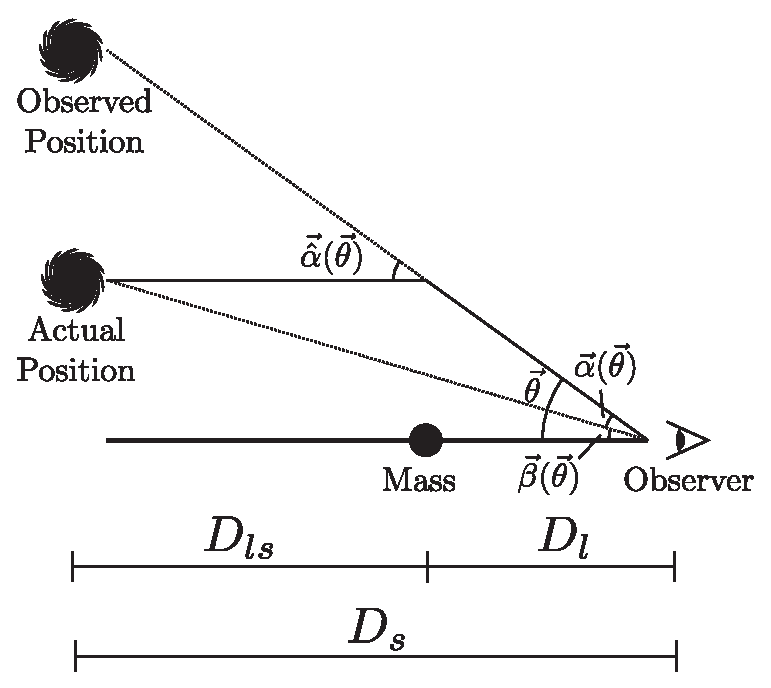
\includegraphics[scale=0.7]{images/lensing_formalism.eps}
\end{figure}

In the thin lens limit, where all the mass is in a single plane $P$ perpendicular to the direction the light is travelling, and between the source and observer. In this limit, we can treat space as Euclidean and find the paths of light as curves within that space that are bent only at a single point. Suppose the mass distribution on $P$ is given by $\Sigma(\v{\xi})$ where $\v{\xi}$ is a \emph{vector} (not a 2-component angle) in $P$. This confusing point is the focus of Section \ref{sec:units}. Then $\v{\alpha}$ is given by \cite{Narayan:1996ba}
\begin{equation}
		\hat{\v{\alpha}}(\v{\xi}) = \frac{4G}{C^2} \int_P \frac{\left( \v{\xi} - \v{\xi}' \right)\Sigma(\v{\xi})}{\n{\v{\xi} - \v{\xi}'}} \, dA
		\label{eq:thin_lens_deflection}
\end{equation}
where $C$ is the speed of light, and $G$ is the gravitational constant, and here $\hat{\v{\alpha}}$ is a vector. The hat is added to distinguish it from the case where it is a scalar. To prevent confusion with lowercase $c$'s that appear later, this document will always use $C$ to refer to the speed of light. $\Sigma$ is referred to as the surface mass density.


Often, the mass distribution will not actually be planar, but will be concenrated near the plane $P$. More precisely, let $z$ be a coordinate parallel to the path of the light. Then the mass distribution is given by $\rho(\v{\xi}, z)$ where $\rho = 0$ for $\n{z} \ge \varepsilon$ where $\varepsilon$ is some distance which is small compared to the distance between the mass and lightsource or the observer. This holds in almost all astronomical situations. In this case, $\Sigma$ is given by integrating $\rho$ over the light of sight:
\begin{equation}
		\Sigma(\v{\xi}) \equiv \int_{-\infty}^\infty \rho(\v{\xi}, z), \, dz.
		\label{eq:LOS_approx}
\end{equation}
This integral will be finite for all $\v{\xi}$ since $\rho(\v{\xi}, \cdot)$ has compact support in the $z$-direction.

In the case where $\Sigma$ is radially symmetric, Equation \eqref{eq:thin_lens_deflection} is simplified greatly. Moving to the coordinate system with the origin at the center of symmetry and applying Gauss's law, the deflection becomes
\begin{equation}
		\hat{\v{\alpha}}(\v{\xi}) =	\hat{\v{\alpha}}(r \hat{\v{r}}) = -\hat{\alpha}(r) \hat{\v{r}}
		\label{eq:radially_symmetric}
\end{equation}
where $r$ is the radial distance from the origin and $\hat{\v{r}}$ is the outward pointing unit normal where
\begin{equation}
		\hat{\alpha}(r) = \frac{4G M(r)}{C^2 r}
		\label{eq:radial_deflection}
\end{equation}
with gravitational constant $G$, $C$ the speed of light, and $M(r)$ the mass enclosed up to radius $r$ from the origin \cite{Narayan:1996ba}. More precisely,
\begin{equation}
		M(r) = \int_0^r \int_0^{2\pi} \Sigma(r') \, r' \, d\theta \, dr' = 2\pi \int_0^r r' \Sigma(r') \, dr'.
		\label{eq:mass_enclosed}
\end{equation}

\section{NFW Profile}

One of the most realistic mass distributions is the NFW profile. This is a fairly accurate approximation for the mass distribution of astronomical objects, including the associated dark matter, across many scales \cite{Navarro:1995iw}. The profile has several dependent parameters, any two of which are sufficient. The parameters chosen depends on the situation at hand. The best source for information about the NFW paper is \cite{brainerd_wright}.

The NFW profile at redshift $z$ is defined to be: \cite{brainerd_wright}
\begin{equation}
		\rho(r) \equiv \frac{\delta_c \rho_c}{(r/r_s)(1+r/r_s)^2}
		\label{eq:NFW_profile}
\end{equation}
where $\delta_c$, $\rho_c$, and $r_s$ are parameters. $\delta_c$ is given by
\begin{equation}
		\delta_c \equiv \frac{200}{3} \frac{c^3}{\ln(1+c) - \frac{c}{1+c}}
		\label{eq:delta_c}
\end{equation}
where $c$ is \emph{NOT} the speed of light, but a unitless parameter of the NFW profile called the concentration. $\delta_c$ is itself unitless. $\rho_c$ is the critical density for closure of the universe at redshift $z$, and has units of mass density. It is given by
\begin{equation}
		\rho_c \equiv \frac{3H^2(z)}{8\pi G}
		\label{eq:rho_c}
\end{equation}
where $H(z)$ is the Hubble constant at redshift $z$, and $G$ is the gravitational constant. Finally, $r_s$ is a characteristic radius for the profile, with units of length and is given by
\begin{equation}
		r_s \equiv \frac{r_{200}}{c}
		\label{eq:r_s}
\end{equation}
where $c$ is again the unitless parameter and $r_{200}$ is the virial radius, i.e. the radius such that the enclosed volume has mass density equal to $200 \rho_c$. The mass enclosed by this radius is given by 
\begin{equation}
		M_{200} \equiv M(r_{200}) = \frac{800 \pi}{3} \rho_c r_{200}^3.
		\label{eq:m_200}
\end{equation}

Of course, this profile is given in three spatial dimensions. To be used with the thin lens approximation, we have to compress it along the light of sight. Let $P$ be some plane through the origin and let $z$ be the line through the origin perpedicular to it. Let $R$ be a radial distance on the plane from the origin. Then $\Sigma(R)$, the surface mass density is given by Equation \eqref{eq:LOS_approx}, except with $R$ instead of $\v{\xi}$ because of radial symmetry. To perform the integration, it is necessary to introduce the dimensionless distance variable $x \equiv R/r_s$. This integral is performed in \cite{brainerd_wright}, giving a complex, but analytic expression.
\begin{equation}
		\Sigma_\text{NFW}(x) = 2r_s \delta_c \rho_c
		\begin{cases}
				\dfrac{1}{x^2-1}\left( 1-\dfrac{2}{\sqrt{1-x^2}} \arctanh \sqrt{\dfrac{1-x}{1+x}}\; \right) & 0 \le x < 1\\[1.2em]
				\dfrac{1}{3} & x=1\\[1.2em]
				\dfrac{1}{x^2-1}\left( 1-\dfrac{2}{\sqrt{x^2-1}} \arctan \sqrt{\dfrac{x-1}{1+x}}\; \right) & 0 \le x < 1\\
		\end{cases}
		\label{eq:NFW_surface_mass_density}
\end{equation}
Although this expression is piecewise, $\Sigma(x)$ is continuous and appears smooth. See the graph below.
\begin{figure}[h]
\center
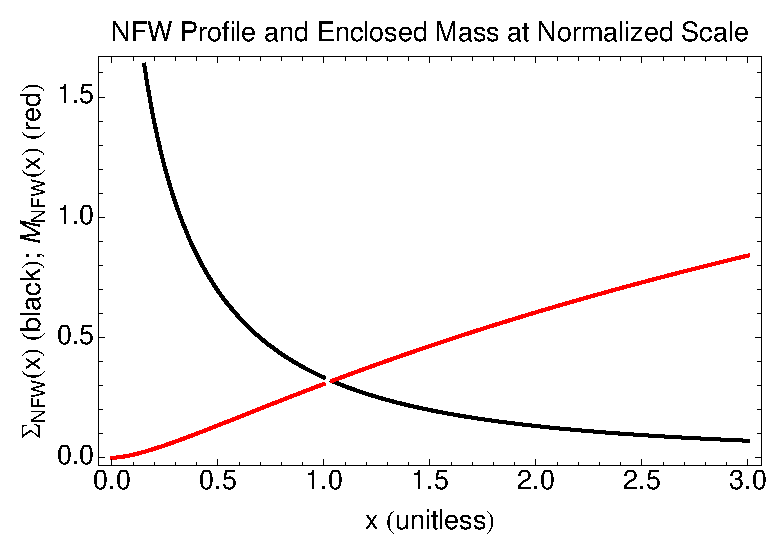
\includegraphics{images/NFW_Profile.eps}
\end{figure}

To find the deflection resulting from this profile, we need to find the enclosed mass, by calculating the integral in \eqref{eq:mass_enclosed}. Luckily, \cite{brainerd_wright} calculates a related quantity, $M(r)/(\pi r^2)$. Working from formula (13) of \cite{brainerd_wright}, we then find
\begin{equation}
		M_\text{NFW}(x) = 
		4 \pi r_s \delta_c \rho_c \left[\ln \frac{x}{2} + 
		\begin{cases}
				\frac{2}{\sqrt{1-x^2}} \arctanh \sqrt{\frac{1-x}{1+x}} & 0 \le x < 1\\[1.2em]
				1 & x = 1\\[1.2em]
				\frac{2}{\sqrt{x^2-1}} \arctanh \sqrt{\frac{x-1}{1+x}} & x > 1
						\end{cases}
						\right].
		\label{eq:NFW_mass_enclosed}
\end{equation}
Inserting this into Equations \eqref{eq:radially_symmetric} and \eqref{eq:radial_deflection} gives the deflection due to an NFW profile.

\section{Units and Implementation}
\label{sec:units}
In the implementation of the simulations, the task is to calculate $\alpha(r)$ given the mass distribution and it's parameters. This is complicated by the plethora of units involved. Fully six different different units of length or position interact in this calculation:
\begin{enumerate}
		\item Two-component angular position (e.g. $\v{\theta}$, $\v{\beta}$, etc).
		\item Two-component vector position (e.g. $\v{\xi}$, $\hat{\v{\alpha}}$, etc).
		\item Angular diameter distance, often measured in megaparsecs (e.g. $D_\ell, D_s, D_{\ell s}$).
		\item Dimensionless units used in the equations for the NFW profile (e.g. $x = R/r_s$).
		\item Image pixels.
		\item Sub-pixels used when tabulating the value of $\alpha(r)$ at different radial distances.
\end{enumerate}


\bibliographystyle{plain}
\bibliography{bib.bib}

\end{document}
